\begin{frame}{Beyond DPO: ORPO and KTO}
  \begin{center}
    \Large
    Beyond DPO: ORPO and KTO
  \end{center}
\end{frame}

\begin{frame}[t]{ORPO: One Stage, No Reference Model}
  \begin{itemize}
    \item[\textcolor{red}{$\blacktriangleright$}] \textbf{Key idea:} DPO removed the reward model but kept two things: a separate SFT stage and a frozen reference policy. ORPO removes both (Hong et al., 2024).
  \end{itemize}

  \vspace{0.3em}
  Define the \textbf{odds} that the model produces $y$ rather than not, and penalise the chosen response's odds being no better than the rejected one's:
  \[
    \mathbf{odds}_\theta(y \mid x) = \frac{P_\theta(y \mid x)}{1 - P_\theta(y \mid x)},
    \qquad
    \mathcal{L}_{\mathrm{OR}} = -\log \sigma\!\left(\log \frac{\mathbf{odds}_\theta(y_w \mid x)}{\mathbf{odds}_\theta(y_l \mid x)}\right)
  \]

  This rides along with the ordinary SFT loss on the chosen response, in a single objective:
  \[
    \mathcal{L}_{\mathrm{ORPO}} = \mathbb{E}_{(x,\,y_w,\,y_l)}\big[\,\mathcal{L}_{\mathrm{SFT}} + \lambda\,\mathcal{L}_{\mathrm{OR}}\,\big]
  \]

  \footnotesize
  There is no $\pi_{\text{ref}}$ anywhere in the expression: one model, one pass, one stage. The authors use $\lambda$ between 0.1 and 0.25 depending on the base model.
\end{frame}

\begin{frame}[t,allowframebreaks]{Why an Odds Ratio}
  \begin{itemize}\itemsep0.4em
    \item[\textcolor{red}{$\blacktriangleright$}] SFT has no mechanism for pushing anything \emph{down}. It raises the likelihood of good answers and is indifferent to bad ones, which is why a second alignment stage was needed at all.
    \item[\textcolor{red}{$\blacktriangleright$}] The odds ratio supplies that missing downward pressure, but gently. Hong et al.\ compare it to the plain probability ratio and find the latter ``leads to more extreme discrimination of the disfavored responses,'' suppressing token logits harder than a model still learning the task can absorb.
    \item[\textcolor{red}{$\blacktriangleright$}] The asymmetry is the whole design: \emph{strong adaptation} toward the chosen response, \emph{weak penalty} on the rejected one. That is what lets alignment share a stage with SFT instead of following it.
    \item[\textcolor{red}{$\blacktriangleright$}] \textbf{What it buys:} one model in memory instead of two or four, and one training run instead of two or three. Mistral-ORPO-$\beta$, trained on UltraFeedback alone, reports 12.20\% on AlpacaEval 2.0 and 7.32 on MT-Bench.
    \item[\textcolor{red}{$\blacktriangleright$}] \textbf{What it costs:} the reference policy was also a leash. Without $\pi_{\text{ref}}$ there is no KL term holding the model near its starting point, so $\lambda$ and the learning rate carry more weight than they do in DPO.
  \end{itemize}
\end{frame}

\begin{frame}{ORPO Against RLHF and DPO}
  \begin{figure}
    \centering
    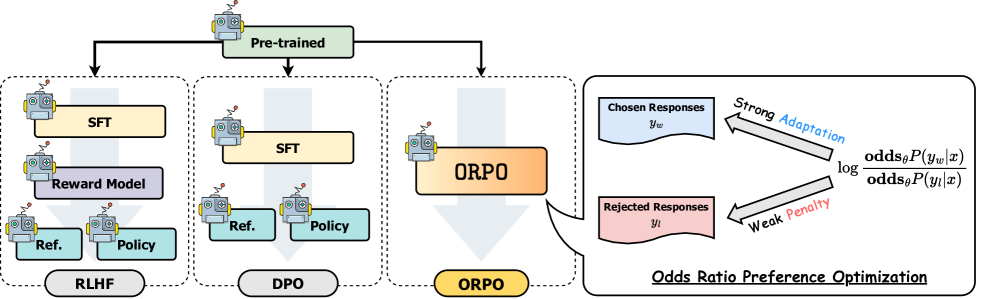
\includegraphics[width=0.88\paperwidth,height=0.46\paperheight,keepaspectratio]{images/llm-rlhf/orpo_vs_rlhf_dpo_pipelines.png}
    \caption*{\scriptsize Hong, Lee \& Thorne, ``ORPO: Monolithic Preference Optimization without Reference Model,'' \href{https://arxiv.org/abs/2403.07691v2}{arXiv:2403.07691v2}, Figure~2.}
  \end{figure}
\end{frame}

\begin{frame}[t]{KTO: Thumbs Up and Thumbs Down}
  \begin{itemize}
    \item[\textcolor{red}{$\blacktriangleright$}] \textbf{The data problem:} PPO, DPO and ORPO all need \emph{pairs}: two responses to the same prompt, ranked. Production systems collect something else: one response, with a thumbs up or down.
    \item[\textcolor{red}{$\blacktriangleright$}] \textbf{KTO} (Ethayarajh et al., 2024) learns from that unpaired signal using the value function from Kahneman and Tversky's prospect theory, which is concave in gains, convex in losses, and measured against a reference point rather than in absolute terms:
  \end{itemize}
  \[
    r_\theta(x,y) = \log \frac{\pi_\theta(y \mid x)}{\pi_{\text{ref}}(y \mid x)},
    \qquad
    z_0 = \mathrm{KL}\big(\pi_\theta(y' \mid x)\,\|\,\pi_{\text{ref}}(y' \mid x)\big)
  \]
  \[
    v(x,y) =
    \begin{cases}
      \lambda_D\,\sigma\big(\beta\,(r_\theta(x,y) - z_0)\big) & \text{if } y \text{ is desirable}\\[0.2em]
      \lambda_U\,\sigma\big(\beta\,(z_0 - r_\theta(x,y))\big) & \text{if } y \text{ is undesirable}
    \end{cases}
    \qquad
    \mathcal{L}_{\mathrm{KTO}} = \mathbb{E}\big[\lambda_y - v(x,y)\big]
  \]

  \footnotesize
  $z_0$ is the model's KL from $\pi_{\text{ref}}$, estimated cheaply from mismatched pairs in the microbatch. $\lambda_y$ is $\lambda_D$ or $\lambda_U$ as $y$ requires; these loss-aversion weights keep $\lambda_D n_D / \lambda_U n_U$ in $[1, 3/2]$, so at a 1:10 desirable-to-undesirable ratio set $\lambda_U = 1$ and $\lambda_D \in [10,15]$. $r_\theta$ still references $\pi_{\text{ref}}$: KTO drops the pairing, not the reference model.
\end{frame}

\begin{frame}[t]{Choosing a Preference Method}
  \begin{center}
    \scriptsize
    \renewcommand{\arraystretch}{1.3}
    \begin{tabular}{|l|>{\raggedright\arraybackslash}p{3.0cm}|c|c|>{\raggedright\arraybackslash}p{3.3cm}|}
      \hline
      \textbf{Method} & \textbf{Data it needs} & \textbf{Models} & \textbf{Stages} & \textbf{Main risk} \\
      \hline
      PPO & Pairs, then prompts to roll out on & 4 & SFT, RM, RL & Instability; reward hacking \\
      DPO & Preference pairs $(x, y_w, y_l)$ & 2 & SFT, then DPO & Sensitive to the SFT starting point \\
      ORPO & Preference pairs $(x, y_w, y_l)$ & 1 & Single stage & No KL leash; $\lambda$ matters more \\
      KTO & Unpaired thumbs up / down & 2 & SFT, then KTO & Needs $\lambda_D, \lambda_U$ set to the class balance \\
      \hline
    \end{tabular}
  \end{center}
  \vspace{0.4em}
  \begin{itemize}
    \item[\textcolor{red}{$\blacktriangleright$}] \textbf{Start from the data you already have, not the leaderboard.} Unpaired feedback points at KTO, which tolerates skew paired methods cannot: discarding 90\% of the desirable data still beat DPO on Llama-7B. Curated pairs on a tight budget point at ORPO; pairs plus an existing SFT model point at DPO.
    \item[\textcolor{red}{$\blacktriangleright$}] PPO stays the most expressive of the four, since it optimises against a reward model rather than a fixed dataset, and the hardest to get right.
  \end{itemize}
\end{frame}
